\documentclass{article}


\usepackage{amsmath}
\usepackage{amssymb}
\usepackage{graphicx}
\usepackage{color}
\usepackage{subfig}
\usepackage{float} % For [H] placement

\usepackage[ruled,vlined,linesnumbered]{algorithm2e}

\usepackage{booktabs}

\usepackage[bookmarks=true,ocgcolorlinks=true,plainpages=false, breaklinks=true, bookmarksopen=true, bookmarksnumbered=true]{hyperref}
%\hypersetup{bookmarks=false}  %hide the bookmarks bar
%\hypersetup{bookmarksopen=false}  % expand tree of bookmarks or just show first level
\hypersetup{linkcolor=blue, citecolor=magenta,urlcolor=blue} % electronic
\hypersetup{colorlinks=true}

\usepackage[T1]{fontenc}
\usepackage{palatino}

\allowdisplaybreaks

\renewcommand{\vec}[1]{\ensuremath{{\boldsymbol #1}}}
\newcommand{\mat}[1]{\ensuremath{\boldsymbol{#1}}}

\newcommand{\unit}[1]{\textcolor{green}{#1}}
\newcommand{\brian}[1]{\textcolor{blue}{#1}}

\title{Statistical performance analysis of neural mass models?}
\date{\today}

\begin{document}


\section{Introduction}
\label{sec:introduction}

Mesoscopic mathematical models of the brain are becoming increasingly popular as tools for generating hypotheses on the physical principals that govern neurodynamics. Forward models have led to theory on the emergence of the brains rhythms, the mechanisms of anesthetic agents, the brains response to sensory stimuli, short-term memory formation, visual hallucinations and epileptic seizures. Most recently, advances engineering methods and computing resources have expanded the utility of these models as integral elements of frameworks to estimate of system and parametric states that can not be directed measured using electrophysiology. An established framework to reliably estimate physical properties underlying brain dynamics has the potential to revolutionise how we observe, diagnose, treat and cure neurological disorders. For example, in epilepsy the dynamics of hidden system and parametric states are thought to be highly patient-specific and unknown. Thus the ability to estimate these quantities using the framework will enable a greater understanding of individuals’ pathologies, leading to more tailored therapies and better patient outcomes.  Furthermore, subject-specific models will enable the application of control theory to the neurosciences, which is typically limited to man-made systems.

To date a large body of work has demonstrated validity of these models in-principal, through the ability to reproduce experimental data. The next stage is understanding the performance of estimation algorithms. Once models have been fit to subjects a final step in assessing validity will be to examine the within subject predictive power.In order for such a framework to be established as a clinical platform further work is required for establishing validity and feasibility for the mesoscopic models. This paper introduces engineering tools to neuroscience community for formally accessing feasibility. We also postulate how these tools can be used to increase performance of estimation methods. 

Influence on sampling rate and estimation?


 


 of this framework History of models and estimation attempts

Usefulness of bound: benchmark algorithms, experimental design, insight about inherent uncertainty -- which do we address


Not claiming anything about which model is the 'best', but simply what level of complexity is possible - how increasing complexity affects uncertainty.
\section{Background}
\label{sec:background}


\paragraph{Neural Mass Model}
\begin{figure}[ht]
  \begin{center}
    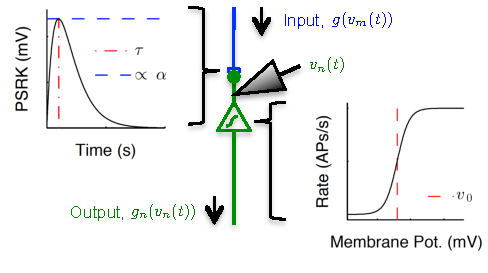
\includegraphics{./figures/pdf/SingleMass_plos.pdf}
  \end{center}
  \caption{\emph{\textbf{Neural Mass Model.} The somas of the neural mass are represented by the triangle. The synaptic connections are represented by the circle. The input mean firing rate, $g(v_m(t))$, is convolved with post-synaptic response kernel (PSRK), shown in the inset on the left, to give the mean membrane potential, $v_n(t)$. This is transformed by the sigmoid, shown in the inset on the right, to give the output mean firing rate, $g(v_n(t))$.}}
  \label{fig:SingleNeuralMass}
\end{figure}
Neural mass models map from a mean firing rate of a population of pre-synaptic neurons to a mean membrane potential of a post-synaptic population, which in turn determines that population's output firing rate. A graphical description of a neural mass model can be seen in Figure~\ref{fig:SingleNeuralMass}. 

To define a standard neural mass model, we begin by defining the post-synaptic potential of population $n$, $v_n(t)$, as a result of an input firing rate from population $m$, $g(v_m(t))$, as the convolution
\begin{equation}\label{eq:conv_eq}
    v_n(t) = \frac{\alpha_{mn}}{\tau_{mn}}\int_{-\infty}^t  h_{mn}(t-t')g(v_m(t')) \,\mathrm{d}t',
\end{equation}
where $\alpha_{mn}$ is the gain for the post-synaptic response kernel (PSRK), denoted by $h_{mn}(t)$, from neural population $m$ to $n$, and $\tau_{mn}$ is the membrane time constant. A common form of the PSRK is
\begin{equation}
    h_{mn}(t) = \eta(t)t\exp\left(-\frac{t}{\tau_{mn}}\right),
\end{equation}
where $\eta(t)$ is the Heaviside step function. An example of a PSRK can be seen in the left inset of Figure~\ref{fig:SingleNeuralMass}.  

The firing rate of each population is related to the mean membrane potential by a sigmoidal activation function; the logistic function sigmoid is typically used: 
\begin{align}
    g\left(v_n(t)\right) =& \frac{1}{1+\exp{\left(\varsigma_n\left(v_{0n} - v_n(t)\right)\right)}}.
    \label{eq:sigmoid}
\end{align}
The quantity $\varsigma_n$ describes the slope of the sigmoid (approximating the variance of firing thresholds within the populations) and $v_{0n}$ describes the mean firing threshold. An example of the sigmoidal activation function can be seen in the right inset of Figure~\ref{fig:SingleNeuralMass}.

The convolution in Equation~\ref{eq:conv_eq} can also be written as the ordinary differential equation (ODE)
\begin{equation}\label{eq:2ndOrder}
    \mathrm{D}v_n(t) = \frac{\mathrm{d}^2 v_n(t)}{\mathrm{d}t^2} + \frac{2}{\tau_{mn}}\frac{\mathrm{d} v_n(t)}{\mathrm{d}t} + \frac{1}{\tau_{mn}^2} v_n(t) = \frac{\alpha_{mn}}{\tau_{mn}} g(v_m(t)),
\end{equation}
where $\mathrm{D}$ is a linear differential operator. Equation~\ref{eq:2ndOrder} can be written as two coupled first-order ODEs by 
\begin{equation} \label{eq:2ndOrderNMM}
    \frac{\mathrm{d} v_n(t)}{\mathrm{d}t} = z_n(t),\,\,\,\,\,    \frac{\mathrm{d}z_n(t)}{\mathrm{d}t} = \frac{\alpha_{mn}}{\tau_{mn}} g(v_m(t)) - \frac{2}{\tau_{mn}}z_n(t) - \frac{1}{\tau_{mn}^2} v_n(t),
\end{equation}
where $z_n(t)$ is a dummy variable. This forms the basis of a state-space model in a canonical format.

The parameters of the model, $\tau$, $\alpha$, $v_0$ and $\varsigma$, can be set so the neural mass has characteristics of specific neural populations, such as pyramidal neurons, spiny stellate cells and fast and slow inhibitory interneurons (GABA$_\mathrm{a}$ and GABA$_\mathrm{b}$). The neural populations can then be connected to represent the circuitry of a cortical column and further to form networks of columns. Various kinds of neural mass models have been developed \cite{Silva1974,Jansen1995,Wendling2002,David2003}, which are depicted in Figure~\ref{fig:NMMs}. Each synaptic connection in these networks can be described by the 2$^{\mathrm{nd}}$-order system of Equation~\ref{eq:2ndOrderNMM}, where the resultant dimensions of the networks of neural mass models in Figures~\ref{fig:NMMs} a, b and c are 6, 12 and 18, respectively.
\begin{figure}[ht]
	\centering
		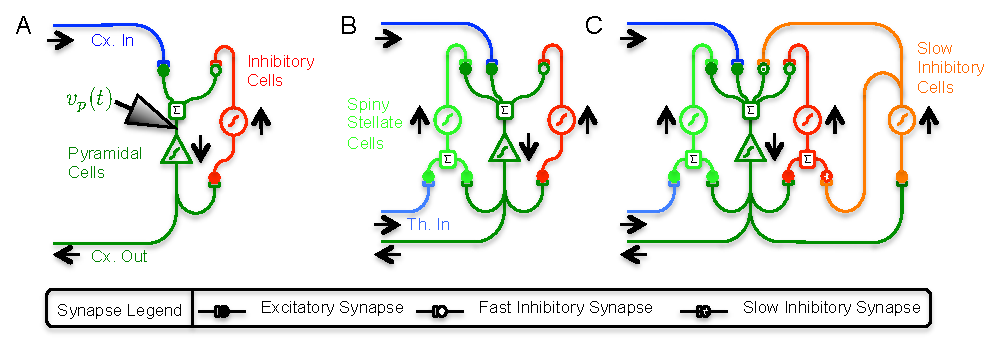
\includegraphics[scale=1]{./figures/pdf/NeuralMassesHoriz_plos.pdf}
	\caption{\emph{\textbf{Models of Cortical Columns.} Each model has a pyramidal neural population, with various forms of feedback and inputs (Cx. = Cortex, Th. = Thalamus). The EEG is taken as the mean membrane potential of the pyramidal population, $v_p(t)$, with additive measurement noise.  a) Minimal model of a column with inhibitory feedback \cite{Silva1974}. b) An extension with excitatory feedback and afferent input from thalamus \cite{Jansen1995,David2003}. c) Column with inhibition occurring across two times scales, enabling modelling of higher frequency activity observed in seizures~\cite{Wendling2002}.}}
	\label{fig:NMMs}
\end{figure}

\begin{figure}[ht]
	\centering
		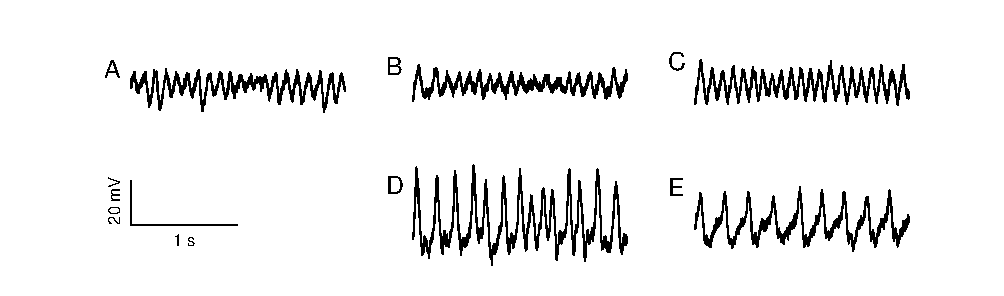
\includegraphics[scale=1]{./figures/pdf/Example_Data.pdf}
		\caption{\textbf{Example data generated using the neural mass models.}}
	\label{fig:NMMs}
\end{figure}


The parameters of the neural masses not only define the population type, but also the behaviour exhibited by the model. For example, certain parameter combinations result in a model of a cortical column that will generate alpha wave type activity (normal activity) and, for another set of parameters, we create a model that will exhibit epileptic behaviour \cite{Wendling2002}. Therefore, we consider a family of models, which we define generally as 
\begin{align}\label{eq:NeuralMassModel}
    \dot{\vec{x}}(t) =& \vec f_{\theta}\left(\vec{x}(t),\vec{u}(t)\right)\\
    y(t) =& \mat{C}\vec{x}(t) + e(t),
\end{align}
where $\vec{x}(t) \in \mathbb{R}^{n_x}$ is a state vector representing the postsynaptic membrane potentials generated by each population synapse and their time derivatives, $n_x$ is the number of states and $\vec{u}(t)$ represents the system input, which may be from afferent connections or other brain regions, exogenous input, or account for model inaccuracies. The function $\vec f_{\theta}(\cdot)$ describes the dynamics, where $\theta \in \mathbb{R}^{n_{\theta}}$ determines the model type and the behaviour it exhibits. The iEEG is denoted by $y(t)$, $\vec{C}$ is the observation matrix, and $e(t)$ is the observation noise.

The model focused on in the following
estimation sections is the formulation by Jansen and Rit \cite{Jansen-Rit-95}.
Given space limitations we refer the reader to the article by Jansen
and Rit\cite{Jansen-Rit-95} where the original state-space equations
are presented. The parameters that were described in this section are related to the Jansen and Rit paper by
\begin{align}
    A =& \frac{\alpha_{pe}}{2e_0c_1} = \frac{\alpha_{pi}}{2e_0c_3} = \frac{\alpha_{ep}}{2e_0c_2} = \frac{\alpha_{xp}}{2e_0} \\
    B =& \frac{\alpha_{ip}}{2e_0c_4} \\
    a =& \frac{1}{\tau_{pe}} = \frac{1}{\tau_{pi}} = \frac{1}{\tau_{ep}} = \frac{1}{\tau_{xp}} \\
    b =& \frac{1}{\tau_{ip}},
\end{align}
where $e_0$ is a parameter that scales the maximum firing rate, $A$ and $B$ are synaptic gains for excitation and inhibition respectively, and $a$ and $b$ are the reciprocals of the synaptic time constants for excitation and inhibition, respectively, and the subscripts $p$, $e$, $x$, and $i$ denote pyramidal ($p$), excitatory interneuron (spiny stellate) ($e$), external ($x$) or inhibitory interneuron ($i$) populations, respectively. By making the assumption that all excitatory synapses share the same time constants and by defining the connectivity constants, $c_1$, $c_2$, $c_3$ and $c_4$, the network of neural masses is the JR NMM.


\section{Theory}

The Bayesian Cramer-Rao bound (BCRB) can be used to examine the inherent uncertainty in a neural mass model and also assess the performance of different estimation algorithms. The bound was formulated in \cite{VanTrees1968} for the estimation of random parameters, making it well suited to the filtering problem described above, where the state is considered a random variable. The BCRB is a lower bound on the mean squared error of an estimator $\hat{\vec x}(\vec y)$ given by
\begin{align}
	\mathsf{MSE} = \mathbb E_{\vec x,\vec y} [(\hat{\vec x}(\vec y) - \vec x)(\hat{\vec x}(\vec y) - \vec x)^T] \ge \mat J^{-1}
	\label{eqn:mse_bound}
\end{align}
where $\mat J$ is the Bayes information matrix defined as
\begin{align}
	\mat J &= -\mathbb E_{\vec x,\vec y}\left[ \nabla_{\vec x}\nabla_{\vec x}^T \log p(\vec y,\vec x) \right] 
	\label{eqn:bayes_matrix}
\end{align}
where $\nabla_{\vec x} = [\partial/\partial x_1,\ldots,\partial/\partial x_n]^T$ and the expectation is taken over the state $\vec x$ and the measurements $\vec y$. 


\subsection{Recursive Bayesian CRB}

To calculate a bound for filtering applications we are required to calculate $\mat J$ defined by \eqref{eqn:bayes_matrix} at each time, $k$. Fortunately, the structure of the joint density $p(\vec y,\vec x)$ allows for a recursive method to calculate $\mat J_k$ from $\mat J_{k-1}$ as demonstrated in \cite{Tichavsky1998}. However, this recursion is not directly applicable to the neural field models described in Section~\ref{sec:background} since noise only enters the system through a single state and the resultant covariance matrix, $\mat Q$, is singular. An alternative recursion proposed in \cite{Bergman2001} is suitable to the models considered here and can be summarised as 
\begin{align}
	\mat J_k = \left( \mat Q + {\mat F}_{k-1} \mat J_{k-1}^{-1} {\mat F}_{k-1}^T\right)^{-1} + \mat C^T \mat R^{-1} \mat C
\end{align}
where
\begin{align}
		{\mat F}_k &= \mathbb E_{\vec x_k} \left[ \nabla_{\vec x_k}^T \vec f(\vec x_k)\right] 
		\label{eqn:F_matrix_expectation}
\end{align}
See Appendix~\ref{sec:derivation_recursion} for details. The expectation over the state $\vec x_k$ in \eqref{eqn:F_matrix_expectation} can rarely be computed in closed form for nonlinear transition functions so Monte Carlo techniques must be employed. A large number of state realisations are generated at each time point and the expectation is approximated by an average over the realisations.

The bound defined above can be used in several ways. Firstly, different models can be compared to test the feasibility of estimating the unknown states from the measurements available. Secondly, different parameter sets can be tested within a single model to assess how the performance of an estimator is expected to change for different types of activity. Finally, the efficiency of a given estimation algorithm (e.g. EKF, particle filter) can be assessed against the lower bound. This indicated whether developing progressively advanced estimation algorithms is warranted, a question that has not been considered in the neural estimation literature thus far.

This paper assumes the parameters of a given model are constant and known. However, it is important to note that the results and conclusions presented in this paper are directly applicable to the case of slowly varying unknown parameters. This statement can be quantified by first considering a state vector that is augmented with constant unknown parameters \cite{sdf}. In this case, the information about the parameters accumulates each time step and the performance bound asymptotically approaches the case for constant known parameters. As an extension, if the parameters are varying slowly with respect to the sampling rate the bound will remain sufficiently close to the case of known parameters.

\section{Simulations}

\subsection{Across models - model feasibility}

We consider the feasibility of the three models described in Section~\ref{sec:background}. Models A and B contain 6 unknown states and model C has 10 unknown states. An important question to ask as the models become increasingly complex is: how well can we estimate the states from the available measurements? To investigate this, we compute the BCRB for each model in an operating mode analogous to alpha rhythms. The specific parameters are listed in Appendix~\ref{sec:parameter_table}.


\subsection{Within model - seizure, alpha}

It has been well demonstrated that models of type B and C can generate vastly different oscillations for different parameters \cite{sdf}. Bifurcation theory provides a theoretical tool to analyse this feature and has been reported in several places \cite{sdf}. Good qualitative agreement between EEG data and the models has been observed and consequently different parameters sets have been assigned to different types of brain activity such as alpha rhythms or epileptic seizures \cite{sfd}.

Here, we investigate ones ability to estimate the states of a model for different types of activity. We calculate the BCRB for model B for two parameter sets representing alpha rhythms and epileptic seizures.

Fig.~\ref{sdf} illustrates that the seizure type behaviour is easier to estimate than background alpha rhythms...<text here>. This is perhaps not surprising since, intuitively, seizure oscillations appear more structured and have larger amplitudes as illustrated in Fig.~\ref{fig:NMMs}.

\subsection{Benchmark algorithms}

EKF doesn't reach bound for any nonlinear model, thus better algorithms are required.

\begin{figure}[ht]
  \begin{center}
    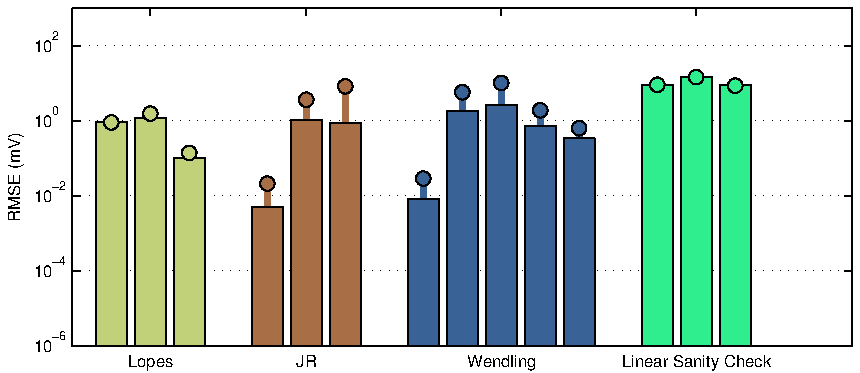
\includegraphics{./figures/pdf/CRBbar}
  \end{center}
  \caption{The mean squared error of the EKF against the BCRB for three models}
  \label{fig:CrbBar}
\end{figure}


\section{Discussion}

extensions to other applications e.g. experimental design

algorithm performance

contextualize work w.r.t. existing literature?

we say nothing about how algorithms will work with uncertainty in the actual model -- thus can be considered a ``best case'' situation, where we know the true model exactly.

\section{Conclusion}

\appendix
\section{Derivation of Recursive Bayesian CRB}\label{sec:derivation_recursion}

The recursion in \cite{Bergman2001} is
\begin{subequations}
\begin{align}
	\mat P_{k|k-1} &= \bar{\mat F}_k\mat P_{k-1|k-1}\bar{\mat F}_k + \bar{\mat G}_k\mat Q_k \bar{\mat G}_k^{-1} \\
		\mat P_{k|k} &= \left(\mat P_{k|k-1}^{-1} + \bar{\mat R}_{k-1}^{-1}\right)^{-1}
\end{align}
\end{subequations}
where
\begin{align}
	\bar{\mat F}_k &= \mathbb E \left[ \nabla_{\vec x_k}^T \tilde{\vec f_k}(\vec x_k,\vec v_k)\right] \\
	\bar{\mat R}_k^{-1} &= -\mathbb E\left[ \nabla_{\vec x_k}\nabla_{\vec x_k}^T \log p(\vec y_k|\vec x_k) \right] \\
	\bar{\mat G}_k &= \mathbb E \left[ \nabla_{\vec v_k}^T \tilde{\vec f_k}(\vec x_k,\vec v_k)\right] \\
	\mat Q_k^{-1} &= -\mathbb E \left[ \nabla_{\vec v_k}\nabla_{\vec v_k}^T \log p(\vec v_k) \right]
\end{align}
and $\mat P_0^{-1}$ is the inverse of the prior covariance. The model in \eqref{eqn:model_general} is represented by $\tilde{\vec f}(\vec x_k,\vec v_k) = \vec f(\vec x_k) + \vec v_k$. This simplifies the derivatives to
\begin{align}
	\nabla_{\vec x_k}^T \tilde{\vec f_k}(\vec x_k,\vec v_k) &= \mat F_k(\vec x_k) \\
	\nabla_{\vec v_k}^T \tilde{\vec f_k}(\vec x_k,\vec v_k) &= \mat I_{d\times d} \\
	\nabla_{\vec x_k}\nabla_{\vec x_k}^T \log p(\vec y_k|\vec x_k) &= -\mat H^T\mat R^{-1} \mat H 
\end{align}
and the corresponding matrices to	
\begin{align}
	\bar{\mat F}_k &= \mathbb E\left[ \mat F_k(\vec x_k)\right] \label{eqn:pcrb_term_F}\\
	\bar{\mat R}_k^{-1} &= \mat H^T\mat R^{-1} \mat H \\
	\bar{\mat G}_k &= \mat I_{d\times d} 
\end{align}
Therefore the final recursion is
\begin{align}
	\mat J_{k|k} = \left( \mat Q + \bar{\mat F}_{k-1} \mat J_{k-1}^{-1} \bar{\mat F}_{k-1}^T\right)^{-1} + \mat H_k^T \mat R^{-1} \mat H_k
\end{align}

\section{List of notation and parameters}
\label{sec:parameter_table}

Table here


\small
\bibliographystyle{ieeetr}
\bibliography{References}




\end{document}
